\documentclass[aspectratio=1610,8pt]{beamer}

% Standard packages

\usepackage[english]{babel}
\usepackage{siunitx}
\usepackage{textcomp}
%\usepackage[latin1]{inputenc}
%\usepackage{times}
%\usepackage[T1]{fontenc}


% Setup TikZ

\usepackage{tikz}
\usetikzlibrary{arrows}
\tikzstyle{block}=[draw opacity=0.7,line width=1.4cm]


% Author, Title, etc.

\title{Doubly Linked List}

\author[Shiv Shankar Dayal]{Shiv Shankar Dayal}

% The main document

\begin{document}
\begin{frame}[fragile]
  \titlepage
\end{frame}
\begin{frame}{Insertion of node at the beginning}
  In the beginning \texttt{head} is \texttt{NULL}. So we allocate a node put
  data in, make its \texttt{prev} pointer \texttt{NULL} and \texttt{next}
  pointer to point to \texttt{head}. Then we make \texttt{head} point to it.
  Let us say data is 10.
  \begin{center}
    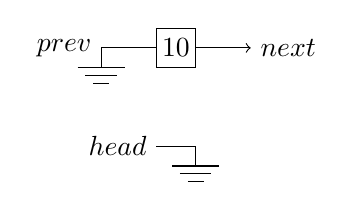
\begin{tikzpicture}
      \draw (0, 0) rectangle(.5, .5);
      \draw (.25, .25) node{$10$};
      \draw (0, .25) -- (-.7, .25) -- (-.7, 0);
      \draw (-1, 0) -- (-.4, 0);
      \draw (-.9, -.1) -- (-.5, -.1);
      \draw (-.8, -.2) -- (-.6, -.2);
      \draw (-.7, .25) node[anchor=east]{$prev$};
      \draw[->] (.5, .25) -- (1.2, .25);
      \draw (1.2, .25) node[anchor=west]{$next$};
      \draw (0, -1) -- (.5, -1) -- (.5, -1.25);
      \draw (0, -1) node[anchor=east]{$head$};
      \draw (.2, -1.25) -- (.8, -1.25);
      \draw (.3, -1.35) -- (.7, -1.35);
      \draw (.4, -1.45) -- (.6, -1.45);
    \end{tikzpicture}
  \end{center}
\end{frame}
\begin{frame}{Insertion of node at the beginning}
  \begin{center}
    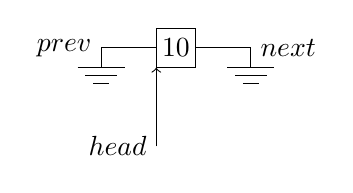
\begin{tikzpicture}
      \draw (0, 0) rectangle(.5, .5);
      \draw (.25, .25) node{$10$};
      \draw (0, .25) -- (-.7, .25) -- (-.7, 0);
      \draw (-1, 0) -- (-.4, 0);
      \draw (-.9, -.1) -- (-.5, -.1);
      \draw (-.8, -.2) -- (-.6, -.2);
      \draw (-.7, .25) node[anchor=east]{$prev$};
      \draw (.5, .25) -- (1.2, .25) -- (1.2, 0);
      \draw (.9, 0) -- (1.5, 0);
      \draw (1, -.1) -- (1.4, -.1);
      \draw (1.1, -.2) -- (1.3, -.2);
      \draw (1.2, .25) node[anchor=west]{$next$};
      \draw (0, -1) node[anchor=east]{$head$};
      \draw[->] (0, -1) -- (0, 0);
    \end{tikzpicture}
  \end{center}
\end{frame}
\begin{frame}{Inserting another node at beginning}
  Out linked list has one node with data 10. Now let us say we want to insert
  another node at beginning with say data 5. The process remains same with one
  change. Since \texttt{head} is not \texttt{NULL} we update \texttt{prev}
  pointer to this new node.
  \begin{center}
    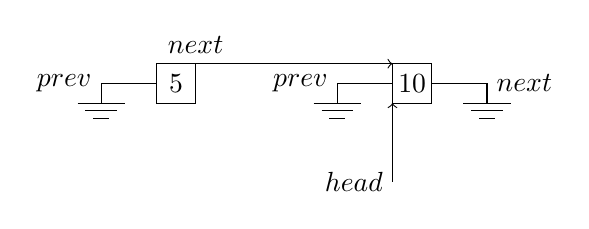
\begin{tikzpicture}
      \draw (0, 0) rectangle(.5, .5);
      \draw (.25, .25) node{$10$};
      \draw (0, .25) -- (-.7, .25) -- (-.7, 0);
      \draw (-1, 0) -- (-.4, 0);
      \draw (-.9, -.1) -- (-.5, -.1);
      \draw (-.8, -.2) -- (-.6, -.2);
      \draw (-.7, .25) node[anchor=east]{$prev$};
      \draw (.5, .25) -- (1.2, .25) -- (1.2, 0);
      \draw (.9, 0) -- (1.5, 0);
      \draw (1, -.1) -- (1.4, -.1);
      \draw (1.1, -.2) -- (1.3, -.2);
      \draw (1.2, .25) node[anchor=west]{$next$};
      \draw (0, -1) node[anchor=east]{$head$};
      \draw[->] (0, -1) -- (0, 0);
      \draw (-3, 0) rectangle(-2.5, .5);
      \draw (-2.75, .25) node{$5$};
      \draw (-3, .25) -- (-3.7, .25) -- (-3.7, 0);
      \draw (-4, 0) -- (-3.4, 0);
      \draw (-3.9, -.1) -- (-3.5, -.1);
      \draw (-3.8, -.2) -- (-3.6, -.2);
      \draw (-3.7, .25) node[anchor=east]{$prev$};
      \draw[->] (-2.5, .5) -- (0, .5);
      \draw (-2.5, .5) node[anchor=south]{$next$};
    \end{tikzpicture}
  \end{center}
\end{frame}
\begin{frame}{Inserting another node at beginning}
  \begin{center}
    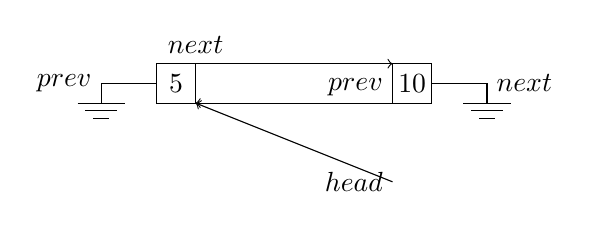
\begin{tikzpicture}
      \draw (0, 0) rectangle(.5, .5);
      \draw (.25, .25) node{$10$};
      \draw[->] (0, 0) -- (-2.5, 0);
      \draw (0, .2) node[anchor=east]{$prev$};
      \draw (.5, .25) -- (1.2, .25) -- (1.2, 0);
      \draw (.9, 0) -- (1.5, 0);
      \draw (1, -.1) -- (1.4, -.1);
      \draw (1.1, -.2) -- (1.3, -.2);
      \draw (1.2, .25) node[anchor=west]{$next$};
      \draw (0, -1) node[anchor=east]{$head$};
      \draw[->] (0, -1) -- (-2.5, 0);
      \draw (-3, 0) rectangle(-2.5, .5);
      \draw (-2.75, .25) node{$5$};
      \draw (-3, .25) -- (-3.7, .25) -- (-3.7, 0);
      \draw (-4, 0) -- (-3.4, 0);
      \draw (-3.9, -.1) -- (-3.5, -.1);
      \draw (-3.8, -.2) -- (-3.6, -.2);
      \draw (-3.7, .25) node[anchor=east]{$prev$};
      \draw[->] (-2.5, .5) -- (0, .5);
      \draw (-2.5, .5) node[anchor=south]{$next$};
    \end{tikzpicture}
  \end{center}
\end{frame}
\begin{frame}{Inserting a node in between}
  Let the data to be inserted is 12. In this case we just manipulate the
  pointers next and previous to the node. First we set the node's \texttt{next}
  and \texttt{prev} pointers and then we adjust the pointers of nodes next and
  previous to it.
  \begin{center}
    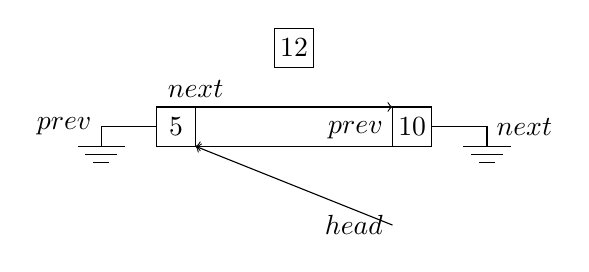
\begin{tikzpicture}
      \draw (0, 0) rectangle(.5, .5);
      \draw (.25, .25) node{$10$};
      \draw[->] (0, 0) -- (-2.5, 0);
      \draw (0, .2) node[anchor=east]{$prev$};
      \draw (.5, .25) -- (1.2, .25) -- (1.2, 0);
      \draw (.9, 0) -- (1.5, 0);
      \draw (1, -.1) -- (1.4, -.1);
      \draw (1.1, -.2) -- (1.3, -.2);
      \draw (1.2, .25) node[anchor=west]{$next$};
      \draw (0, -1) node[anchor=east]{$head$};
      \draw[->] (0, -1) -- (-2.5, 0);
      \draw (-3, 0) rectangle(-2.5, .5);
      \draw (-2.75, .25) node{$5$};
      \draw (-3, .25) -- (-3.7, .25) -- (-3.7, 0);
      \draw (-4, 0) -- (-3.4, 0);
      \draw (-3.9, -.1) -- (-3.5, -.1);
      \draw (-3.8, -.2) -- (-3.6, -.2);
      \draw (-3.7, .25) node[anchor=east]{$prev$};
      \draw[->] (-2.5, .5) -- (0, .5);
      \draw (-2.5, .5) node[anchor=south]{$next$};
      \draw (-1, 1) rectangle (-1.5, 1.5);
      \draw (-1.25, 1.25) node{$12$};
    \end{tikzpicture}
  \end{center}
\end{frame}
\end{document}
